%% Default Latex document template
%%
%%  blake@rcs.ee.washington.edu

\documentclass[letterpaper]{article}

% Uncomment for bibliog.
%\bibliographystyle{unsrt}

\usepackage{graphicx}
\usepackage{amsmath}
%\usepackage{fancyhdr}

%%%%%%%%%%%%%%%%%%%%%%%%%%%%%%%%%%%%%%%%5
%
%  Set Up Margins
\input{templates/pagedim.tex}

%
%        Font selection
%
%\renewcommand{\rmdefault}{ptm}             % Times
%\renewcommand{\rmdefault}{phv}             % Helvetica
%\renewcommand{\rmdefault}{pcr}             % Courier
%\renewcommand{\rmdefault}{pbk}             % Bookman
%\renewcommand{\rmdefault}{pag}             % Avant Garde
%\renewcommand{\rmdefault}{ppl}             % Palatino
%\renewcommand{\rmdefault}{pch}             % Charter


%%%%%%%%%%%%%%%%%%%%%%%%%%%%%%%%%%%%%%%%%%%%%%%%%
%
%         Page format Mods HERE
%
%Mod's to page size for this document
\addtolength\textwidth{0cm}
\addtolength\oddsidemargin{0cm}
\addtolength\headsep{0cm}
\addtolength\textheight{0cm}
%\linespread{0.894}   % 0.894 = 6 lines per inch, 1 = "single",  1.6 = "double"

% header options for fancyhdr

%\pagestyle{fancy}
%\lhead{LEFT HEADER}
%\chead{CENTER HEADER}
%\rhead{RIGHT HEADER}
%\lfoot{Hannaford, U. of Washington}
%\rfoot{\today}
%\cfoot{\thepage}



% Make table rows deeper
%\renewcommand\arraystretch{2.0}% Vertical Row size, 1.0 is for standard spacing)

\begin{document}

\begin{center}\Large{Combinatorics-based method for derivation of solution sets for
Inverse Kinematics}

\today
\end{center}

\section{}
One of our main learnings in this project is that robot kinematic equation solutions in general are NOT described by a tree structure! Instead they are a more general graph. For example, two variable solutions might be independent of each other but contribute to the other variables' solutions (multiple 'roots' to the graph). Our previous solution was overly complex due to lingering assumptions from the tree structure idea.
We have done a complete re-write of the solution set generator process with seemingly good results. The key insight was to develop the table of solutions, adding rows as each solved variable creates combinations.

In the new approach, for each solved variable, we distinguish between the number of ``solutions” and the number of
``versions” it has.  The number of solutions is determined by the mathematical form of the
solution for example:

\beq
x=\sin{(\theta)}
\eeq
\noindent
has two solutions (and also two versions).
\beq
\theta =[\arcsin(x), \pi-\arcsin(x)]
\eeq

However a variable whose solution is single valued, could have multiple versions of it depends on a variable with multiple versions.  For example,
\beq
y = \theta + \pi
\eeq
\noindent
$y$ has one solution, but two versions
\beq
y = [\pi + \arcsin(x) , 2\pi - \arcsin(x)]
\eeq
depending on which version of $ \theta$ is used.  We identify previously solved unknowns (such as $x$)
appearing in
the right hand side of solution equations as ``dependencies".

In general, an unknown may have multiple solutions to its equation, and may have more than one dependency,
and all the combinations of versions of the dependencies
generate  versions of the current variable.
To summarize, if a variable has $n_s$ solutions and $n_d$  combinations of its dependencies,
Then it has $n_s \times n_d$ versions.  If a variable $x_i$ has $m$ different variables as dependencies, then
it as

\beq\label{VersionProductEqn}
n_{vi} = n_{sj} \Pi_{j=1}^{m} n_{vj}
\eeq

Note that we have studied this problem solely for the case of $n_{sj} \in \{ 1,2\}$.

We illustrate this with  a small system of equations which is easy to solve but has these
versioning characteristics
of IK problems.
Let the problem  be to find all sets of the unknowns $[x_1 \dots x_5]$ which satisfy the following five equations.

\beq\label{X1Eqn}
x_1 - x_4 - x_2 = 0
\eeq

\beq
x_2 - x_4/2 = 0
\eeq

\beq
9-x_3 = 0
\eeq

\beq\label{X4Eqn}
x_4 - \sqrt{x_3} =0
\eeq

\beq\label{X5Eqn}
\sqrt{4} - x_5 = 0
\eeq

where each of the $x_i$ are unknowns and the other terms (here they are numbers) are known.
By inspection, we can solve these in the order  $[(x_3, x_5)(tie), x_4, x_2, x_1 ]$.

\begin{enumerate}
\item $x_3$ is a trivial solution: $x_3=9$ and there is only one solution.
\item $x_5$ is simple, but there are two solutions: $[\sqrt{4}, -\sqrt{4}]$.
\item $x_4$ similarly has two solutions:  $[\sqrt{9}, -\sqrt{9}]$.
\item $x_2$ has only one solution, $x_4/2$, but we have two {\it versions} due
to the two solutions of $x_4$: $[1.5,-1.5]$
\item $x_1$ depends on both $x_4$ and $x_2$ so though it has one solution, it
has four versions (in general distinct): $[4.5, -4.5, -4.5, 4.5]$ due to the
combinations of versions of its two dependencies.
\end{enumerate}

\vspace{0.1in}
\begin{center}
\begin{tabular}{c|c|c}
var.,    & multiplicity  &  Solutions or Versions\\\hline
$x_3$    &   1    & $[9]$\\
$x_5$    &   2    & $[2,-2]^S$\\
$x_4$    &   2    & $[3,-3]^S$\\
$x_2$    &   1    & $[1.5,-1.5]^V$\\
$x_1$    &   1    & $[4.5,-4.5,-4.5,4.5]^V$\\
\end{tabular}
\end{center}
\vspace{0.1in}


The solutions dependencies can be represented as a graph (Figure \ref{graphFig}), but unlike a tree,
the graph is not especially helpful in finding the solution sets.

\begin{figure}\centering
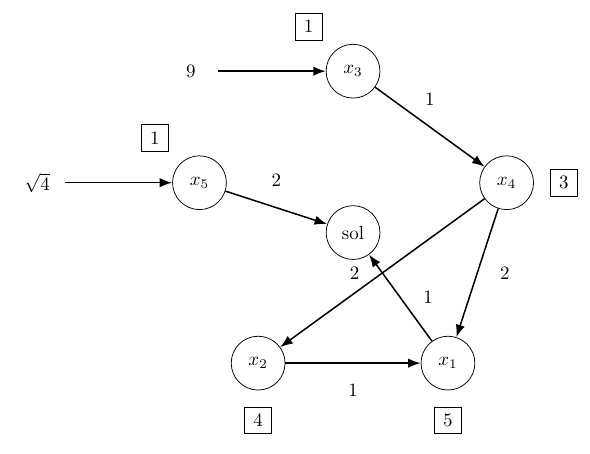
\includegraphics[width=0.5\linewidth]{solutionGraph.png}
\caption{Dependencies to solution of Equations \ref{X1Eqn} to \ref{X5Eqn}.   Edge weights are
         $n_{si}$ of the origin of the edge.  The square annotation gives the solution order of each variable.
         ``sol" node is the full solution set. }\label{graphFig}
\end{figure}

 Next, we assemble solution vectors by following the solution order as follows:

\begin{enumerate}
  \item $x_3$ has one solution, $x_{3s1}=9$ giving one  version
  \beq
  x_{3v1} = x_{3s1} = 9
  \eeq
  We will continue by collecting these versions into a set of vectors:
    \beq
    \begin{bmatrix}
    x_{3v1}
    \end{bmatrix}
    \eeq
  \item $x_5$ has two solution but depends on no previous unknowns.  Its versions are thus
  $x_{5v1}=x_{5s1} = 2, x_{5v2}=x_{5s2} = -2$.   We thus double the number of rows giving:
    \beq
    \begin{bmatrix}
           x_{3v1}   & x_{5v1}  \\
           x_{3v1}   & x_{5v2}  \\
    \end{bmatrix}
    \eeq
  note that the order of these two variable columns does't matter since they are independent of each other.

  \item $x_4$ has two solutions based on the multiple solutions of
  Eqn \ref{X4Eqn} which depend on $x_3$ (having only one version) but
  these solutions are independent of $x_4$
  and $x_5$.  We thus have to double the rows again and we have to flip the order of the newly
  added rows to generate the full set of combinations:
    \beq
    \begin{bmatrix}
           x_{3v1}   & x_{5v1}  &  x_{4v1}\\
           x_{3v1}   & x_{5v2}  &  x_{4v2}\\
           x_{3v1}   & x_{5v2}  &  x_{4v1}\\
           x_{3v1}   & x_{5v1}  &  x_{4v2}\\
    \end{bmatrix}
    \eeq
  \item $x_2$, similarly has one solution (so we do not double the rows)
  but depends on the versions of $x_4$ so it has 4 versions.

    \beq
    \begin{bmatrix}
           x_{3v1}   & x_{5v1}  &  x_{4v1}  & x_{2v1} \\
           x_{3v1}   & x_{5v2}  &  x_{4v2}  & x_{2v2} \\
           x_{3v1}   & x_{5v2}  &  x_{4v1}  & x_{2v3} \\
           x_{3v1}   & x_{5v1}  &  x_{4v2}  & x_{2v4} \\
    \end{bmatrix}
    \eeq

    \item $x_1$ has only one solution, but it depends on two variables:
      $x_2$ which has 2 versions, and $x_4$ which has two versions.
      Applying Eqn \ref{VersionProductEqn}. we have 4 versions:
      \beq
      \begin{aligned}
          x_{1v1} &= x_{4v1} + x_{2v1} \\
          x_{1v2} &= x_{4v2} + x_{2v2} \\
          x_{1v3} &= x_{4v1} + x_{2v3} \\
          x_{1v4} &= x_{4v2} + x_{2v4} \\
      \end{aligned}
      \eeq
    but we do not increase the number of rows because of the single solution to Eqn \ref{X1Eqn}.
    \beq
    \begin{bmatrix}
           x_{3v1}   & x_{5v1}  &  x_{4v1}  & x_{2v1} & x_{1v1} \\
           x_{3v1}   & x_{5v2}  &  x_{4v2}  & x_{2v2} & x_{1v2} \\
           x_{3v1}   & x_{5v2}  &  x_{4v1}  & x_{2v3} & x_{1v3}\\
           x_{3v1}   & x_{5v2}  &  x_{4v2}  & x_{2v4} & x_{1v4} \\
    \end{bmatrix}
    \eeq

\end{enumerate}


The above process can be summarized as:

Once an algorithm such as IKBT has found solutions to all $n_u$ unknowns we can then collect valid
solution vectors into an $n_u \times n_v$ matrix as follows:

\noindent
For each variable $x_i$ in solution order:
\begin{enumerate}
  \item Determine its number of solutions from its solution method. Example: $\sqrt{x}$ has 2 solutions)
  \item Determine its number of dependencies on previously solved unknowns and determine
  the number of versions of each dependency: $n_{vj}$.  Example: $y_5(y_2, y_4)$ where
  $y_2$ has 4 versions and $y_4$ has 2 versions.
  \item Compute the number of versions for $x_i$, $n_{vi}$,  using Eqn \ref{VersionProductEqn}.
  \item If the new number of versions is a multiple of the $n_d$ per  Eqn \ref{VersionProductEqn}, then
  repeat the previous rows  $n_{si}$ times, but flip their order\footnote{Open Issue:
  Understood so far only for $n_{sj} \in \{ 1,2\}$.
  If a variable had e.g. 4 solutions, how to flip the quadrupled rows??}.
  \item Number the versions $x_{ivj}$ where $i$ selects the variable and $j$ selects the
  version number.
  \item Enumerate and save the expression for each  version.  For example: if the solutions are
     \begin{itemize}
        \item $x_{4s1} = -\sqrt{9}$
        \item $x_{4s2} =  \sqrt{9}$
     \end{itemize}
     Then renumber them by row number $x_{4vi}$ and add them as a new column to the solution vector matrix.
  If $n_{si}$ is less than the number of versions, $n_{vi}$,
  copy the solutions $n_{di}$ times and append them to to get $n_{vj}$ rows.
\end{enumerate}

%
% \section{Solution Graphs}
%
% A graph of the solution dependncies can be constructed.   For the system of equations above, and
% the solution list, we have

%  this verbal graph description was used with ChatGPT to get a start on the graph tikz code.
% Five nodes, $x_1 \dots x_2$.  The graph is a directed graph such that if an edge points from $N1$ to $N2$ then $N2$ depends on $N1$.  Weights are tagged on the edges giving the number of solutions.
%  The edges are:  x3 points to x4 (weight 1), x4 points to x2 (weight 2), x4 points to
% x1 (weight 2), x2 points to x1 (weight 1).   Nodes x5, x1 have little edges that point to a node
% labeled "sol." such that x5 points to sol (weight 2) and x1 points to sol (weight 1).
% Nodes x5 and x3 have input edges coming from math symbols:  $\sqrt{4}$ points to x5,
% 9 points to x3.    Finally, each node is labed with a digit inside a square box:
%   x1 [5], x2 [ 4] , x3 [ 1] , x4 [ 3] , x5 [ 1].   Can you please create latex code for this
%   graph?


%  Use name of bibliography files without .bib extension
%\bibliography{brl}
\end{document}

